% Apertura del capítulo 1: sobre una lámina curva no hay ejes cartesianos globales;
% la base tangente (g₁, g₂) y la normal cambian de punto a punto.
% Compilar con: scripts/compilar_tikz.sh   (→ figures/svg/apertura-cap01-bases.svg)
% Superficie ilustrativa z = A sin(k x) cos(k y); los vectores tangentes son exactos
% (g₁ = (1,0,h_x), g₂ = (0,1,h_y), n = g₁×g₂/|g₁×g₂|), escalados para el dibujo.
\def\pgfsysdriver{pgfsys-dvisvgm.def}
\documentclass[tikz,border=0pt]{standalone}
\usetikzlibrary{calc}
\definecolor{lo}{HTML}{1D4ED8}   % azul del libro
\definecolor{hi}{HTML}{0E7490}   % verde azulado del libro
\definecolor{g1c}{HTML}{1D4ED8}
\definecolor{g2c}{HTML}{15803D}
\definecolor{nc}{HTML}{B45309}
\begin{document}
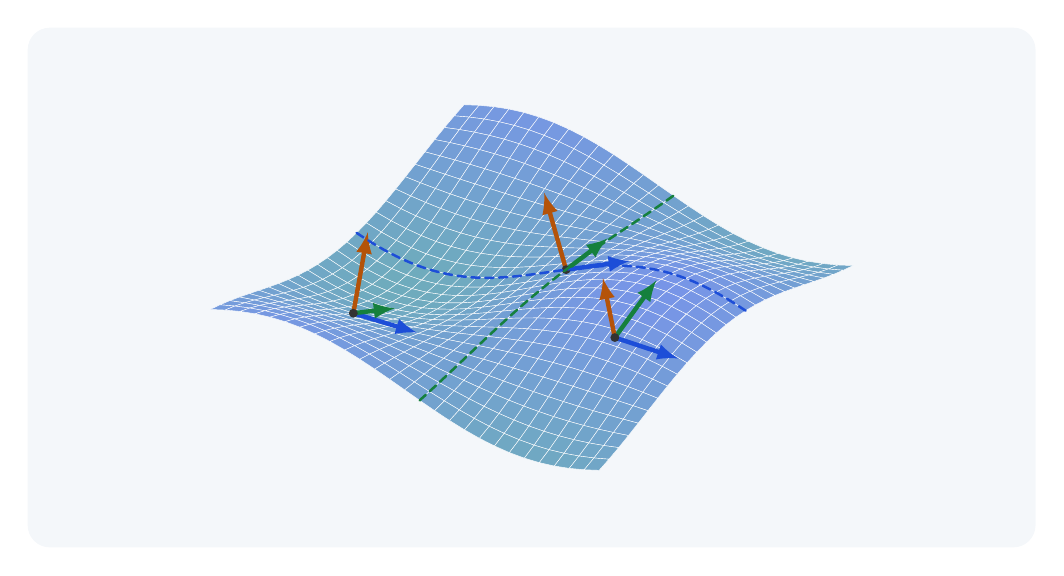
\begin{tikzpicture}[x={(0.95cm,-0.30cm)}, y={(0.62cm,0.50cm)}, z={(0cm,1.1cm)}, line join=round, line cap=round]
  \pgfmathsetmacro{\A}{0.45}
  \pgfmathsetmacro{\k}{0.95}     % radianes
  \pgfmathsetmacro{\L}{2.6}
  \pgfmathsetmacro{\N}{26}
  \pgfmathsetmacro{\h}{2*\L/\N}
  \useasboundingbox (canvas cs:x=-6.4cm,y=-3.3cm) rectangle (canvas cs:x=6.4cm,y=3.3cm);
  \fill[rounded corners=8pt, fill={rgb,255:red,244;green,247;blue,250}]
    (canvas cs:x=-6.4cm,y=-3.3cm) rectangle (canvas cs:x=6.4cm,y=3.3cm);
  % Superficie, de atrás hacia delante
  \foreach \j in {\numexpr\N-1\relax,...,0}{
    \foreach \i in {0,...,\numexpr\N-1\relax}{
      \pgfmathsetmacro{\xa}{-\L+\i*\h}  \pgfmathsetmacro{\xb}{\xa+\h}
      \pgfmathsetmacro{\ya}{-\L+\j*\h}  \pgfmathsetmacro{\yb}{\ya+\h}
      \pgfmathsetmacro{\za}{\A*sin(\k*\xa r)*cos(\k*\ya r)}
      \pgfmathsetmacro{\zb}{\A*sin(\k*\xb r)*cos(\k*\ya r)}
      \pgfmathsetmacro{\zc}{\A*sin(\k*\xb r)*cos(\k*\yb r)}
      \pgfmathsetmacro{\zd}{\A*sin(\k*\xa r)*cos(\k*\yb r)}
      \pgfmathsetmacro{\t}{50+50*(\za+\zb+\zc+\zd)/(4*\A)}
      \fill[lo!\t!hi!60!white, draw=white, line width=0.15pt]
        (\xa,\ya,\za) -- (\xb,\ya,\zb) -- (\xb,\yb,\zc) -- (\xa,\yb,\zd) -- cycle;
    }
  }
  % Tres puntos con su triada local (g1, g2, normal)
  \foreach \u/\v in {-1.6/-1.2, 0.2/0.4, 1.7/-0.9}{
    \pgfmathsetmacro{\z}{\A*sin(\k*\u r)*cos(\k*\v r)}
    \pgfmathsetmacro{\hx}{\A*\k*cos(\k*\u r)*cos(\k*\v r)}
    \pgfmathsetmacro{\hy}{-\A*\k*sin(\k*\u r)*sin(\k*\v r)}
    \pgfmathsetmacro{\nn}{sqrt(1+\hx*\hx+\hy*\hy)}
    \pgfmathsetmacro{\s}{0.85}
    \draw[g1c, -latex, line width=1.6pt] (\u,\v,\z) -- ({\u+\s},\v,{\z+\s*\hx});
    \draw[g2c, -latex, line width=1.6pt] (\u,\v,\z) -- (\u,{\v+\s},{\z+\s*\hy});
    \draw[nc,  -latex, line width=1.6pt] (\u,\v,\z) -- ({\u-\s*\hx/\nn},{\v-\s*\hy/\nn},{\z+\s/\nn});
    \fill[black!80] (\u,\v,\z) circle (1.6pt);
  }
  % Líneas coordenadas θ¹ y θ² que pasan por el punto central
  \draw[g1c, line width=0.9pt, densely dashed, domain=-\L:\L, samples=60] plot (\x,0.4,{\A*sin(\k*\x r)*cos(\k*0.4 r)});
  \draw[g2c, line width=0.9pt, densely dashed, domain=-\L:\L, samples=60] plot (0.2,\x,{\A*sin(\k*0.2 r)*cos(\k*\x r)});
\end{tikzpicture}
\end{document}
